\documentclass{article}
\usepackage{graphicx}
\usepackage{amsthm}
% \usepackage[yyyymmdd]{datetime}
\theoremstyle{definition}
\usepackage{mathtools}
\usepackage{natbib}
\usepackage{thmtools}
\usepackage[usenames, dvipsnames]{color}

\newtheorem{example}{Example}
\newtheorem{theorem}{Theorem}

\declaretheoremstyle[headfont=\bfseries]{solution}
\declaretheoremstyle[headfont=\normalfont]{normalhead}
\declaretheorem[style=normalhead, numbered=no]{question}
\declaretheorem[style=normalhead, numbered=no]{instance}
\declaretheorem[style=solution, numbered=no]{solution}

\title{The Traveller's Problem}
\author{Iva Babukova}

\begin{document}
\maketitle

\section{Use Cases}
\label{npcompleteproblems}

\textcolor{red}{This Section gives a list of known NP-complete problems \citep{thebible} referred to in this work when proving NP-hardness of TP (Section \ref{npcompleteproof}) and as use cases when reviewing the existing work (Section \ref{sec:existingwork}).}

\begin{enumerate}
\item \textbf{Travelling Salesman Problem (TSP)}

\begin{instance}
Set $A$ of $n$ cities, distance $d(A_{i}, A_{j})$ between each pair of cities $A_{i}$, $A_{j}$ $\in$ $A$ \textcolor{red}{that satisfies the triangle inequality}, positive integer $B$.
\end{instance}

\begin{question}
Is there a tour of $A$ having length $B$ or less, i.e., a permutation of cities $\gamma = A_{\pi(1)}, A_{\pi(2)},...,A_{\pi(n)}$ of $A$ such that
$$\bigg( \sum_{i=1}^{n-1} d(A_{\pi(i)}, A_{\pi(i+1)}) \bigg) + d(A_{\pi(n)}, A_{\pi(1)}) \leq B \quad \textrm{?}$$
\end{question}

\item \textbf{Time-Constrained TSP (TCTSP)}

\begin{instance}
Set $A$ of $n$ cities, distance d($A_{i}$, $A_{j}$) between each pair of cities $A_{i}$, $A_{j}$ $\in$ $A$, positive integer $B$, lower and upper bounds $l_{i}$ and $u_{i}$ respectively for each city $A_{i}$ that specify its time window.
\end{instance}

\begin{question}
It there a TSP tour such that for each city $A_{i}$ visited at time $t_{i}$, $l_{i} \leq t_{i} \leq u_{i}$ ?
\end{question}

% \item \textbf{Vehicle-Routing Problem (VRP)}
% \item \textbf{Job-Shop Scheduling Problem (JSSP)}
% \item \textbf{Longest Path Problem}
\end{enumerate}


\section{Complexity of TP}

We state a theorem about the complexity of TP and prove it.

\begin{theorem}
The decision version of TP is NP-complete.
\end{theorem}

\begin{proof}
\label{npcompleteproof}
This proof first shows the membership of TPD in the NP class of problems. Second, we prove the NP-hardness of TP by constructing a polynomial-time reduction from a known NP-complete problem $\Pi$ to TPD, where $\Pi$ is chosen to be the traveling salesman problem (TSP), defined in Section \ref{npcompleteproblems}. Its NP-hardness follows by a reduction from the Hamiltonian Cycle problem. The proof is presented by \cite{thebible}.

Given an instance of TPD and $s$, which is a sequence of flights from $F$, we can write an algorithm $V$ that checks in polynomial time whether $s$ is a solution. To accept or reject validity, $V$ only needs to traverse $s$ and check that it satisfies all required properties. Therefore, TP is in NP.

Let $\pi$ be an instance of TSP, as defined in Section \ref{npcompleteproblems}. Let $\pi^{\prime}$ be an instance of TPD with the following properties:
\begin{itemize}
\item The set of airports in $\pi^{\prime}$ is identical to the set of cities in $\pi$ and it is similarly denoted as $A$ (a city in $\pi$ is called an airport in $\pi^{\prime}$).
\item Each airport in $A$ is also a destination.
\item $T$ is equal to $n+1$.
\item \textcolor{red}{Let $C$ be the Cartesian product of the airports in $A$ with itself, that is $C = A \times A$ = \{($A_{i}, A_{j}$) : $A_{i}$ $\in$ $A$, $A_{j}$ $\in$ $A$, $i \neq j$\}. Then $F$ is a set of flights, such that for every ($A_{i}, A_{j}$) $\in$ $C$, there exists a flight $f_{k}$ in $F$, such that $A^{d}_{k} = A_{i}$ and $A^{a}_{k} = A_{j}$ for every date $t \leq T$.}
\item For every $f_{k}$ $\in$ $F$, $c_{k}$ is equal to $d(A^{d}_{k}, A^{a}_{k})$ in $\pi$. \textcolor{red}{Therefore, the flights cost also satisfies the triangle inequality.} 
\item For every $f_{k}$ $\in$ $F$, $\Delta_{k}$ = 1.
\item $B$ is the upper bound on the allowed total cost.
\end{itemize}

%% TSP solution => also TP solution
\textcolor{red}{
Suppose that $\gamma$ = $A_{i_{1}}, A_{i_{2}},...,A_{i_{n}}$ is the most optimal solution of $\pi$, where $<i_{1},...,i_{n}>$ is a permutation of $<1,...,n>$ and the total travel distance $L_{\gamma} \leq B$. In $\pi^{\prime}$, $\gamma$ is equivalent to the order of visited airports by some sequence of flights $s$ = $f_{i_{1}}, f_{i_{2}},...f_{i_{n}}$, such that for every $f_{i_{k}} \in s, 1 \leq k \leq n$:}

\begin{itemize}
\color{red}
\item $ A^{d}_{i_{k}} = A_{i_{k}}, A_{i_{k}} \in \gamma $, and
\item $ A^{a}_{i_{k}} = A_{i_{k+1}}$, where subscripts are taken modulo $n$.
\end{itemize}

From the two conditions above it follows that $s$ satisfies property 1 and 2 of a valid solution. To satisfy property 3 and 4, it is sufficient to choose flights from $F$ such that for every $f_{k}$ $\in$ $s$, $t{k}$ = $k$. We know that such flights exist in $F$ by the construction of the set $F$. Property 5 is satisfied, since all airports in $A$ are destinations. Therefore, $s$ is a solution of $\pi^{\prime}$, from which it follows that a solution of $\pi$ is also a solution of $\pi^{\prime}$.

%% TP solution => also TSP solution
\textcolor{red}{Suppose that $s = \{f_{j_{1}},...,f_{j_{m}}\}$ is the most optimal solution of $\pi^{\prime}$, where flights in $s$ visit destinations in the sequence $\gamma^{\prime}$ = $\{A_{i_{1}}, A_{i_{2}},...,A_{i_{n}}\}$. We will prove that $\gamma^{\prime}$ is a solution of $\pi$. 
By construction of $\pi^{\prime}$, $\gamma^{\prime}$ contains all airports in A.
Suppose that an arbitrary airport $A_{s}$, for $i_{1} \leq s < i_{n}$, is included more than once in $\gamma^{\prime}$. Therefore, $A_{s}$ is listed at least twice in the tour: $\gamma^{\prime} = \{A_{i_{1}},...,A_{s-1},A_{s},...,A_{p},A_{s},A_{p+1}\}$ for $s < p < i_{n}$ and $s=\{f_{i_{1}},...,f_{q},f_{q+1},...,f_{i_{m}}\}$. The tour is shown in Figure \ref{fig:routes}, where the green circles represent the airports, the red and black arrows are flights in $s$ and the purple flight $f_{r}$ in in $F$, but not in $s$. Since $s$ is the most optimal solution, $c_{q} + c_{q+1} < c_{r}$. However, by construction of $\pi^{\prime}$ the cost of the flights satisfies the triangle inequality and $c_{q} + c_{q+1}$ must be greater than $c_{r}$. This is a contradiction. Therefore, $A_{s}$ can not be added more than once to $\gamma^{\prime}$. Since $A_{s}$ was arbitrary chosen, the tour contains each airport in $A$ exactly once, which makes it a valid solution to $\pi$. Therefore, the most optimal solution of $\pi^{\prime}$ is a solution of $\pi$.}

\begin{figure}
\centering
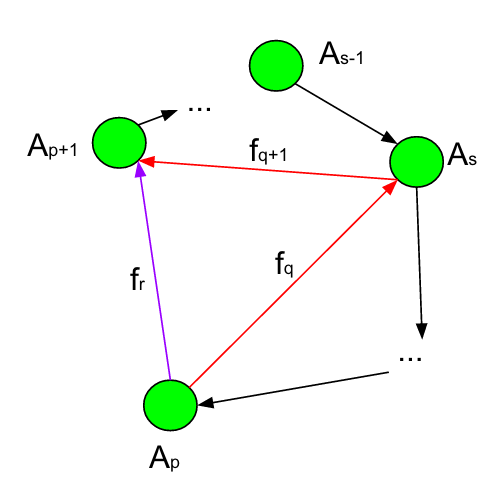
\includegraphics[width=6cm, height=6cm]{images/routes.png}
\label{fig:routes}
\caption{Tour $\gamma^{\prime}$}
\end{figure}

The transformation from a TSP instance to an instance of TPD can be done in polynomial time. For each of the $n$($n$-1)/2 distances d($A_{i}$, $A_{j}$) that must be specified in $\pi$, it is sufficient to check that the same cost is assigned to the flights from $A_{i}$ to $A_{j}$ for all dates.

Therefore, TP is in NP and the decision version of TSP can be reduced to TPD in polynomial time, from which it follows that TPD is NP-complete.

\end{proof}
%%%%%%%%%%%%%%%%%%%%
%   BIBLIOGRAPHY   %
%%%%%%%%%%%%%%%%%%%%

\bibliographystyle{plainnat}
\bibliography{bib}

\end{document}







